\section[P. de movimientos]{Planeación de movimientos}

\begin{frame}\frametitle{Planeación de movimientos}
  El problema de la planeación de movimientos comprende cuatro tareas básicas:
  \begin{itemize}
  \item Navegación (encontrar una ruta por el espacio libre de un punto inicial a uno final). Si la ruta está parametrizada con repecto al tiempo, se dice que es una trayectoria.
  \item Mapeo (construir una representación del ambiente a partir de las lecturas de los sensores y la configuración)
  \item Localización (determinar la configuración a partir de un mapa y de lecturas de los sensores)
  \item Barrido (pasar un actuador por todos los puntos de un subespacio)
  \end{itemize}
  Comúnmente el mapeo y la localización se realizan al mismo tiempo en el proceso conocido como SLAM (\textit{Simultaneous Localization and Mapping})
\end{frame}

\begin{frame}\frametitle{Celdas de ocupación}
  Es una discretización del espacio con una resolución determinada donde a cada celda se le asigna un número $p\in[0,1]$ que indica su nivel de ocupación.
  \begin{itemize}
  \item En un enfoque probabilístico, $p$ indica la certeza de que la celda esté ocupada: 0, certeza de que está libre, 1, certeza de que está ocupada, 0.5, no se tiene información.
  \item En este curso, los niveles de ocupación solo serán 0 o 1.
 Para evitar el manejo de flotantes, el nivel de ocupación suele representarse con un entero en el intervalo [0,100] y un -1 si no hay información. 
  \end{itemize}
  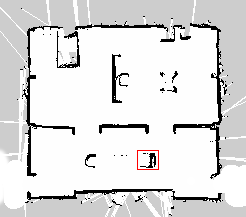
\includegraphics[width=0.4\textwidth]{Figures/OccupancyGrid.png}
  
\includegraphics[width=0.4\textwidth]{Figures/OccupancyGridZoom.png}
\end{frame}

\begin{frame}[containsverbatim]\frametitle{Ejercicio}
  Ejecute el comando:
  \begin{lstlisting}
    roslaunch bring_up path_planning.launch
  \end{lstlisting}
  Inspeccione el mapa en el visualizador RViz. Luego abra el archivo:
  \texttt{catkin\_ws/src/config\_files/maps/appartment.pgm}
  con cualquier editor de imágenes y modifíquelo.
  \\Detenga la ejecución y vuelva a correr el comando anterior. 
\end{frame}

\begin{frame}\frametitle{Planeación de rutas}
  Dado un espacio de configuraciones $Q$ con espacio libre $Q_{free}\subset Q$ y espacio ocupado $Q_{occ}\subset Q$, la planeación de rutas consiste en contrar un mapeo:
  \[f: [0,1] \rightarrow Q_{free} \qquad \textrm{con}\qquad f(0) = q_s\qquad f(1)=q_g\]
  donde $q_s$ y $q_g$ son las configuraciones inicial y meta, respectivamente. Es decir, se debe encontrar una secuencia de puntos del espacio libre que permitan al robot moverse del punto inicial al punto meta sin chocar. Los métodos para planear rutas se pueden agrupar en:
  \begin{itemize}
  \item Basados en búsqueda en grafos (A*, Dijkstra)
    \begin{itemize}
    \item En un mapa de celdas de ocupación, cada celda es un nodo del grafo.
    \item Cada nodo está conectado con las celdas vecinas del espacio libre. 
    \end{itemize}
  \item Basados en muestreo (RRT)
  \item Variacionales
  \end{itemize}
\end{frame}

\begin{frame}\frametitle{El algoritmo A*}
    \begin{algorithm}[H]
    \footnotesize
    \DontPrintSemicolon
    \KwData {Mapa $M$ de celdas de ocupación, configuración inicial $q_{start}$, configuración meta $q_{goal}$}
    \KwResult{Ruta $P=[q_{start},q_1, q_2, \dots , q_{goal}]$}
    Obtener los nodos $n_s$ y $n_g$ correspondientes a $q_{start}$ y $q_{goal}$\;
    Lista abierta $OL = \emptyset$ y lista cerrada $CL = \emptyset$\;
    \ForAll{Nodo $n \in M$}
    {
      $g(n) = \infty$\;
      $f(n) = \infty$\;
    }
    Agregar $n_s$ a $OL$\;
    $g(n_s) = 0$\\
    $f(n_s) = 0$\\
    Nodo actual $n_c = n_s$\;
    \While{$OL\neq \emptyset$ y $n_c\neq n_g$}
    {
      Seleccionar de $OL$ el nodo $n_c$ con el menor valor $f$\;
      Agregar $n_c$ a $CL$\;
      Expandir $n_c$\;
      Agregar a $OL$ los vecinos de $n_c$ que no estén ya en $OL$ ni en $CL$\;
    }
    \If{$n_c\neq n_g$}{Anunciar Falla}
    Obtener la configuración $q_i$ para cada nodo $n_i$ de la ruta\;
  \end{algorithm}
\end{frame}

\begin{frame}[containsverbatim]\frametitle{Ejercicio}
    \lstinputlisting[language=Python]{Codes/AStar.py}
\end{frame}
